\chapter{Automatic Extraction of Landmarks: Analysis}
In this chapter, we present some generic concepts of image processing and a method to automatic extraction landmarks from biological images.
\section{Landmarks}
\textit{``Morphological landmarks are points that can be located precisely and establish an ambiguous one-to-one correspondence among all the specimens and are widely used in shape analysis"}\cite{bookstein1997morphometric}. The fields of shape analysis by landmarks are increasing, especially it really useful in biological and medical field. From the position of the landmarks, we can estimate the size of the object and classify the object into groups. The anatomical landmarks can be collected in two dimensions image. The coordinate of landmarks are usually obtained by manually. This work can take a long time. To solve this problems, we focused on a method to automatic extraction of landmarks. This method based on the article:\textbf{``Automatic indentification of landmarks in digital images"}, which proposed by Palaniswamy. It includes 4 steps:
\begin{enumerate}
\item Segmentation: including preprocessing image and extracting the features,
\item Construction and comparison the Pairwise Geometric Histogram,
\item Estimation the global pose of object by the Probabilistic Hough Transform,
\item Refinement the estimated landmarks by template matching.
\end{enumerate}
\section{Segmentation}
Segmentation is a process to extract interested features from the digital image. The expected result in this stage is the list of approximate lines which are presented for the image's features.\\
The process is mainly separated into two steps: firstly, we pre-process image to reduce the noise and enhance the quality of features in image. Secondly, we extract the image's features (edges) and present it as list of approximate lines.
\subsection{Pre-process image}
Pre-process image decrease the noises and enhance the features in image. The requirement of this step is making an image without the noises and retaining the features in image. To finish the pre-processing step, we apply the \textbf{threshold} method for this reason. This way is different with the suggested method in the article\cite{palaniswamy2010automatic} (DoG filter) to pre-process image. Usually, the threshold value might indicated follows two ways: manually and automatically. In our case, the threshold value was indicated by analysing the image histogram. The method to indicate the threshold value will be focused in next chapter.
\begin{figure}[h!]
\centering
\subfloat[Image with noise]{\label{fig:seg_211}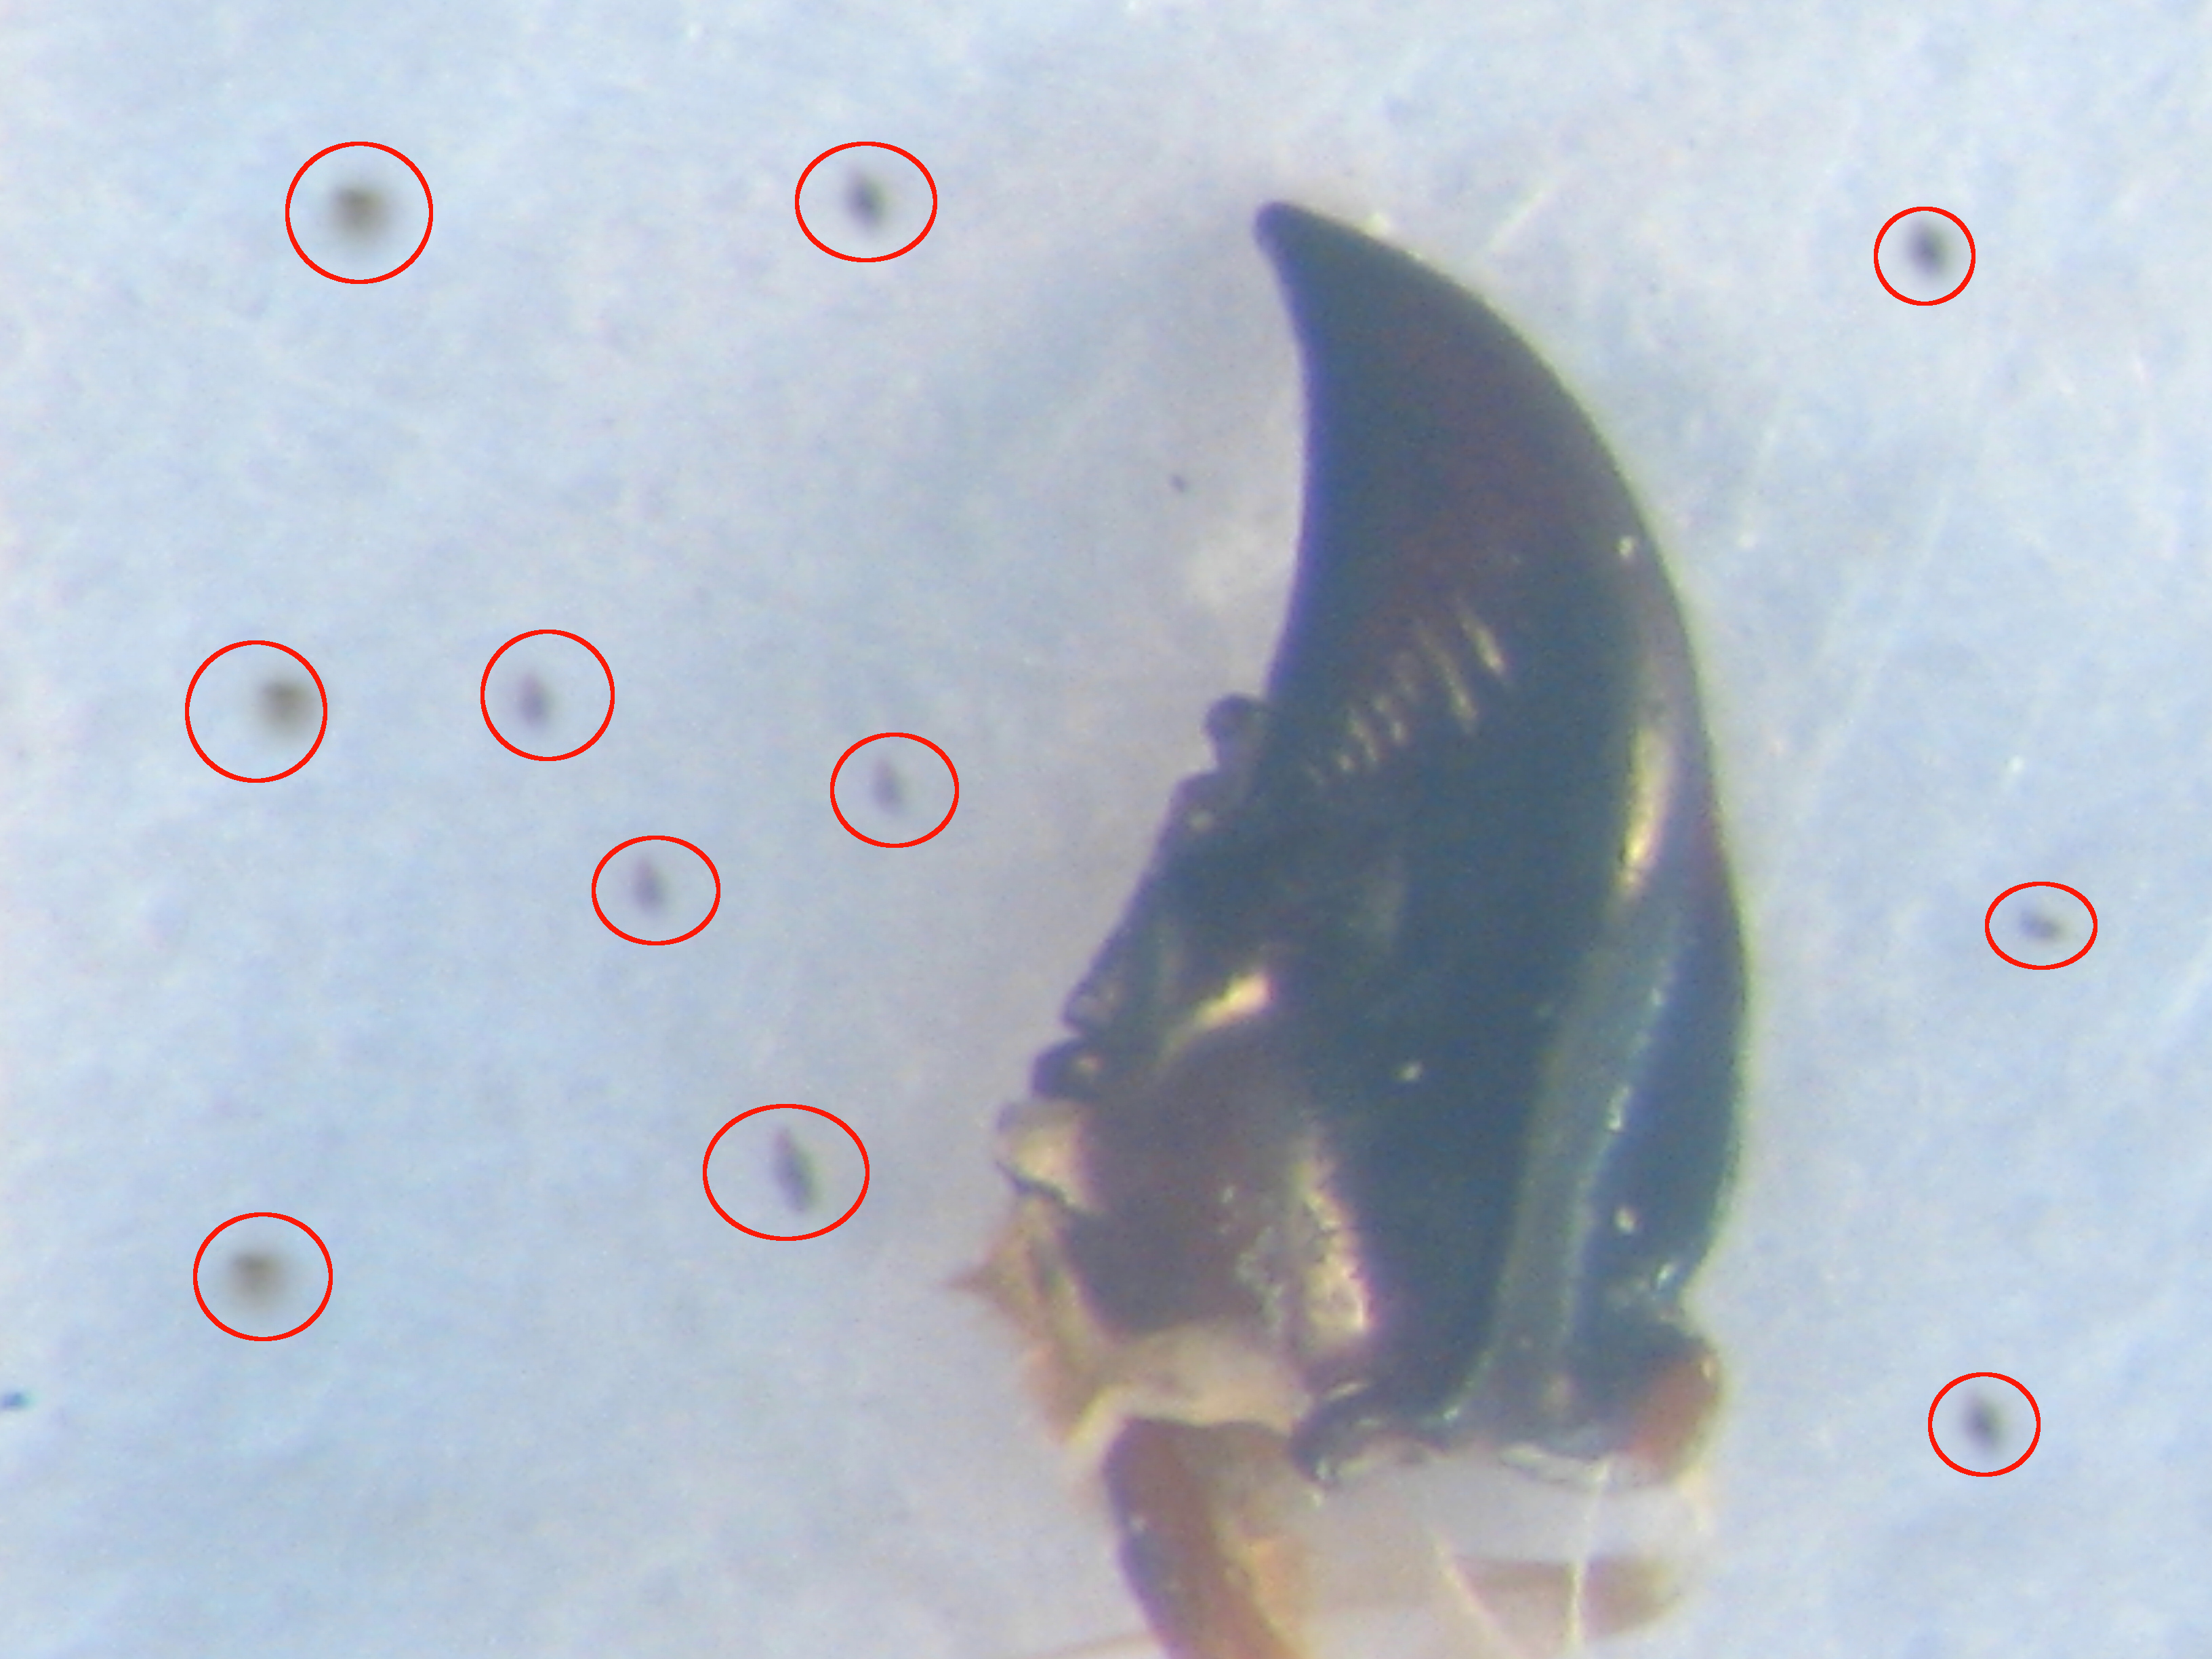
\includegraphics[width=0.45\textwidth]{./images/md019n}}~~
\subfloat[Image without noises]{\label{fig:seg_212}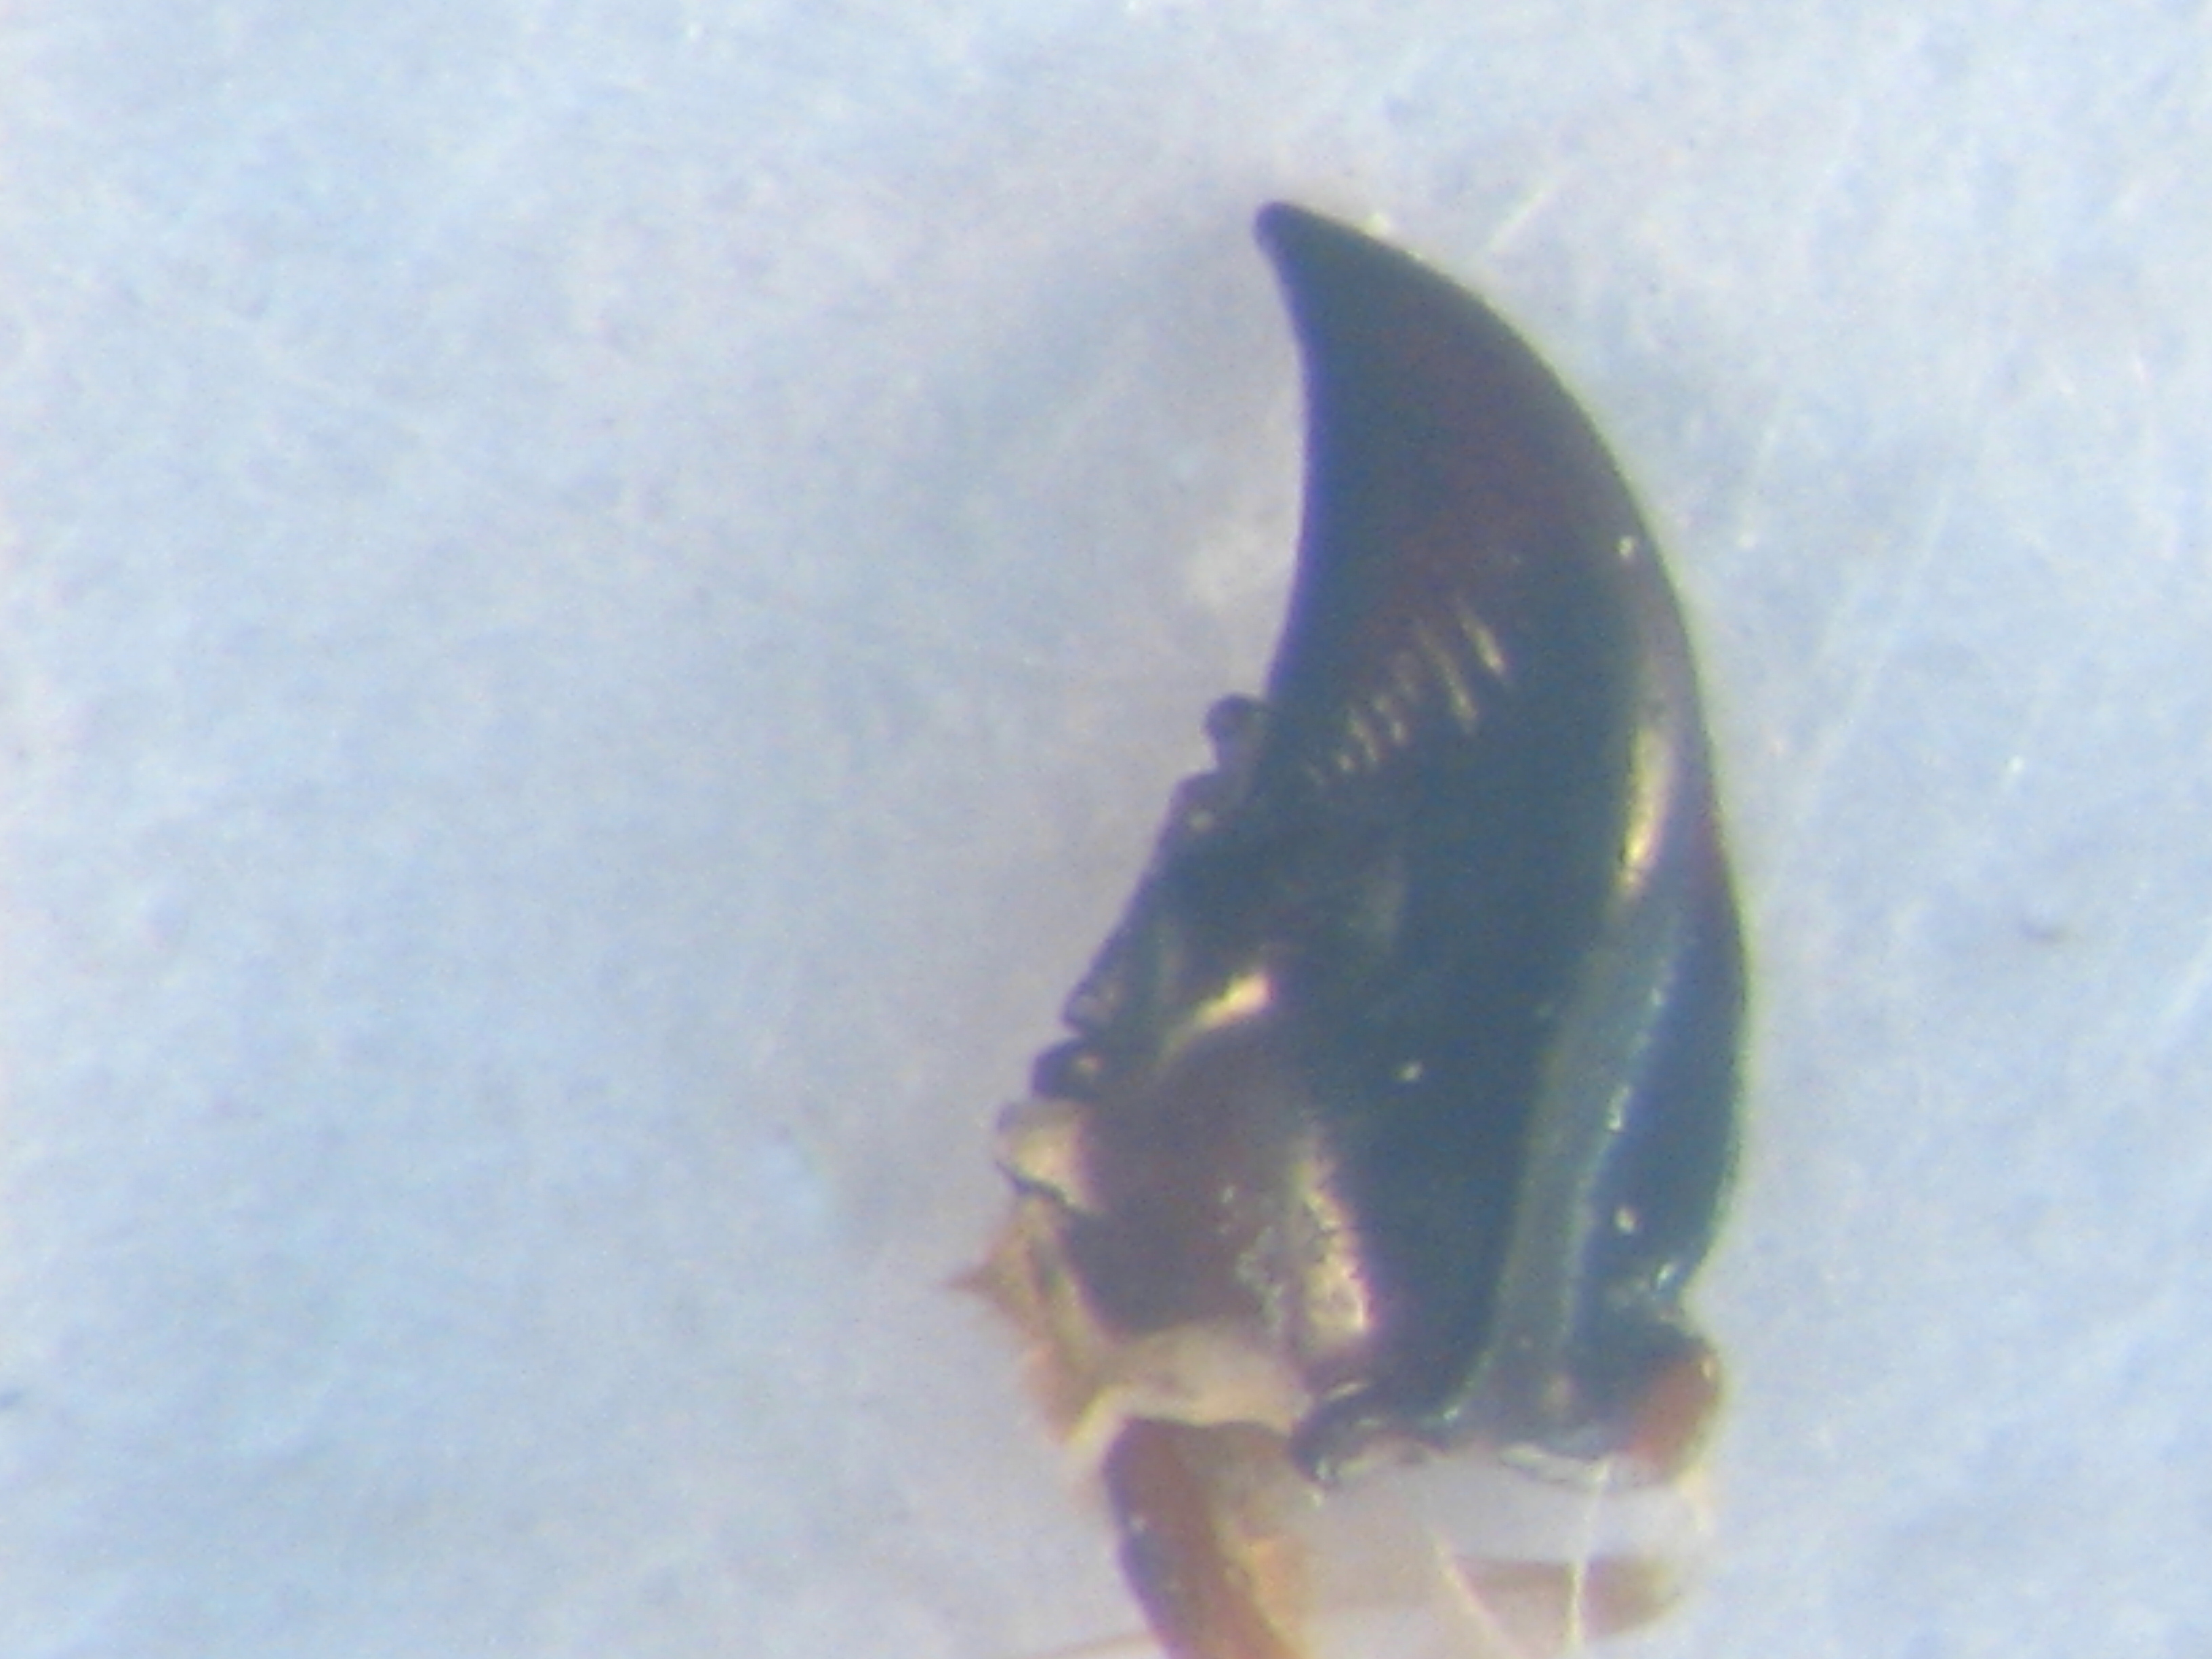
\includegraphics[width=0.45\textwidth]{./images/md019no}}
\caption{Example about noises in image}
\label{fig:figure_21}
\end{figure}
\subsection{Feature extraction}
The Canny\cite{canny1986computational} algorithm, which incorporates non-maximal suppression and hysteresis thresholding, is used to detect the edges. In Canny algorithm, the important parameters are the two threshold values (\textit{lower threshold} and \textit{upper threshold}) because it will decide which pixels are kept. Normally, the value of lower threshold and upper threshold are determined according to a certain rate of the threshold values. \\
Actually, the Canny algorithm is not aware of the actual edges, the edge detecting process was based on the Sobel operator, extracted with non-maximal suppression. To obtain the expecting result, we need to apply another technique to obtain the step edges. In this case, we can use the technique to analysis the structure of topology to get the edges. This technique was proposed by Suzuki\cite{suzuki1985topological} which indicates two borders of the object in binary image (outer border and inner border) based on the relations the borders of a binary image. 
\subsection{Edge segmentation}
The geometric relation of an object could not be constructed from edges, it is always constructed from the relation of basic geometric objects, such as the lines.  In fact, any arbitrary edge can be represented by a set of approximate lines. This presentation is useful when we want to describe the relationship between the edges in an object. The method used to fragment the edge into a list of approximate lines is the recursive algorithm\cite{thacker1995assessing}, which is a new improved version with the method proposed by Lowe\cite{lowe1987three} except the stop condition changed. An example about edge segmentation is presented in figure \ref{fig:figure_22} by using \cite{thacker1995assessing}.
\begin{figure}[h!]
\centering
\subfloat[Original image]{\label{fig:seg_221}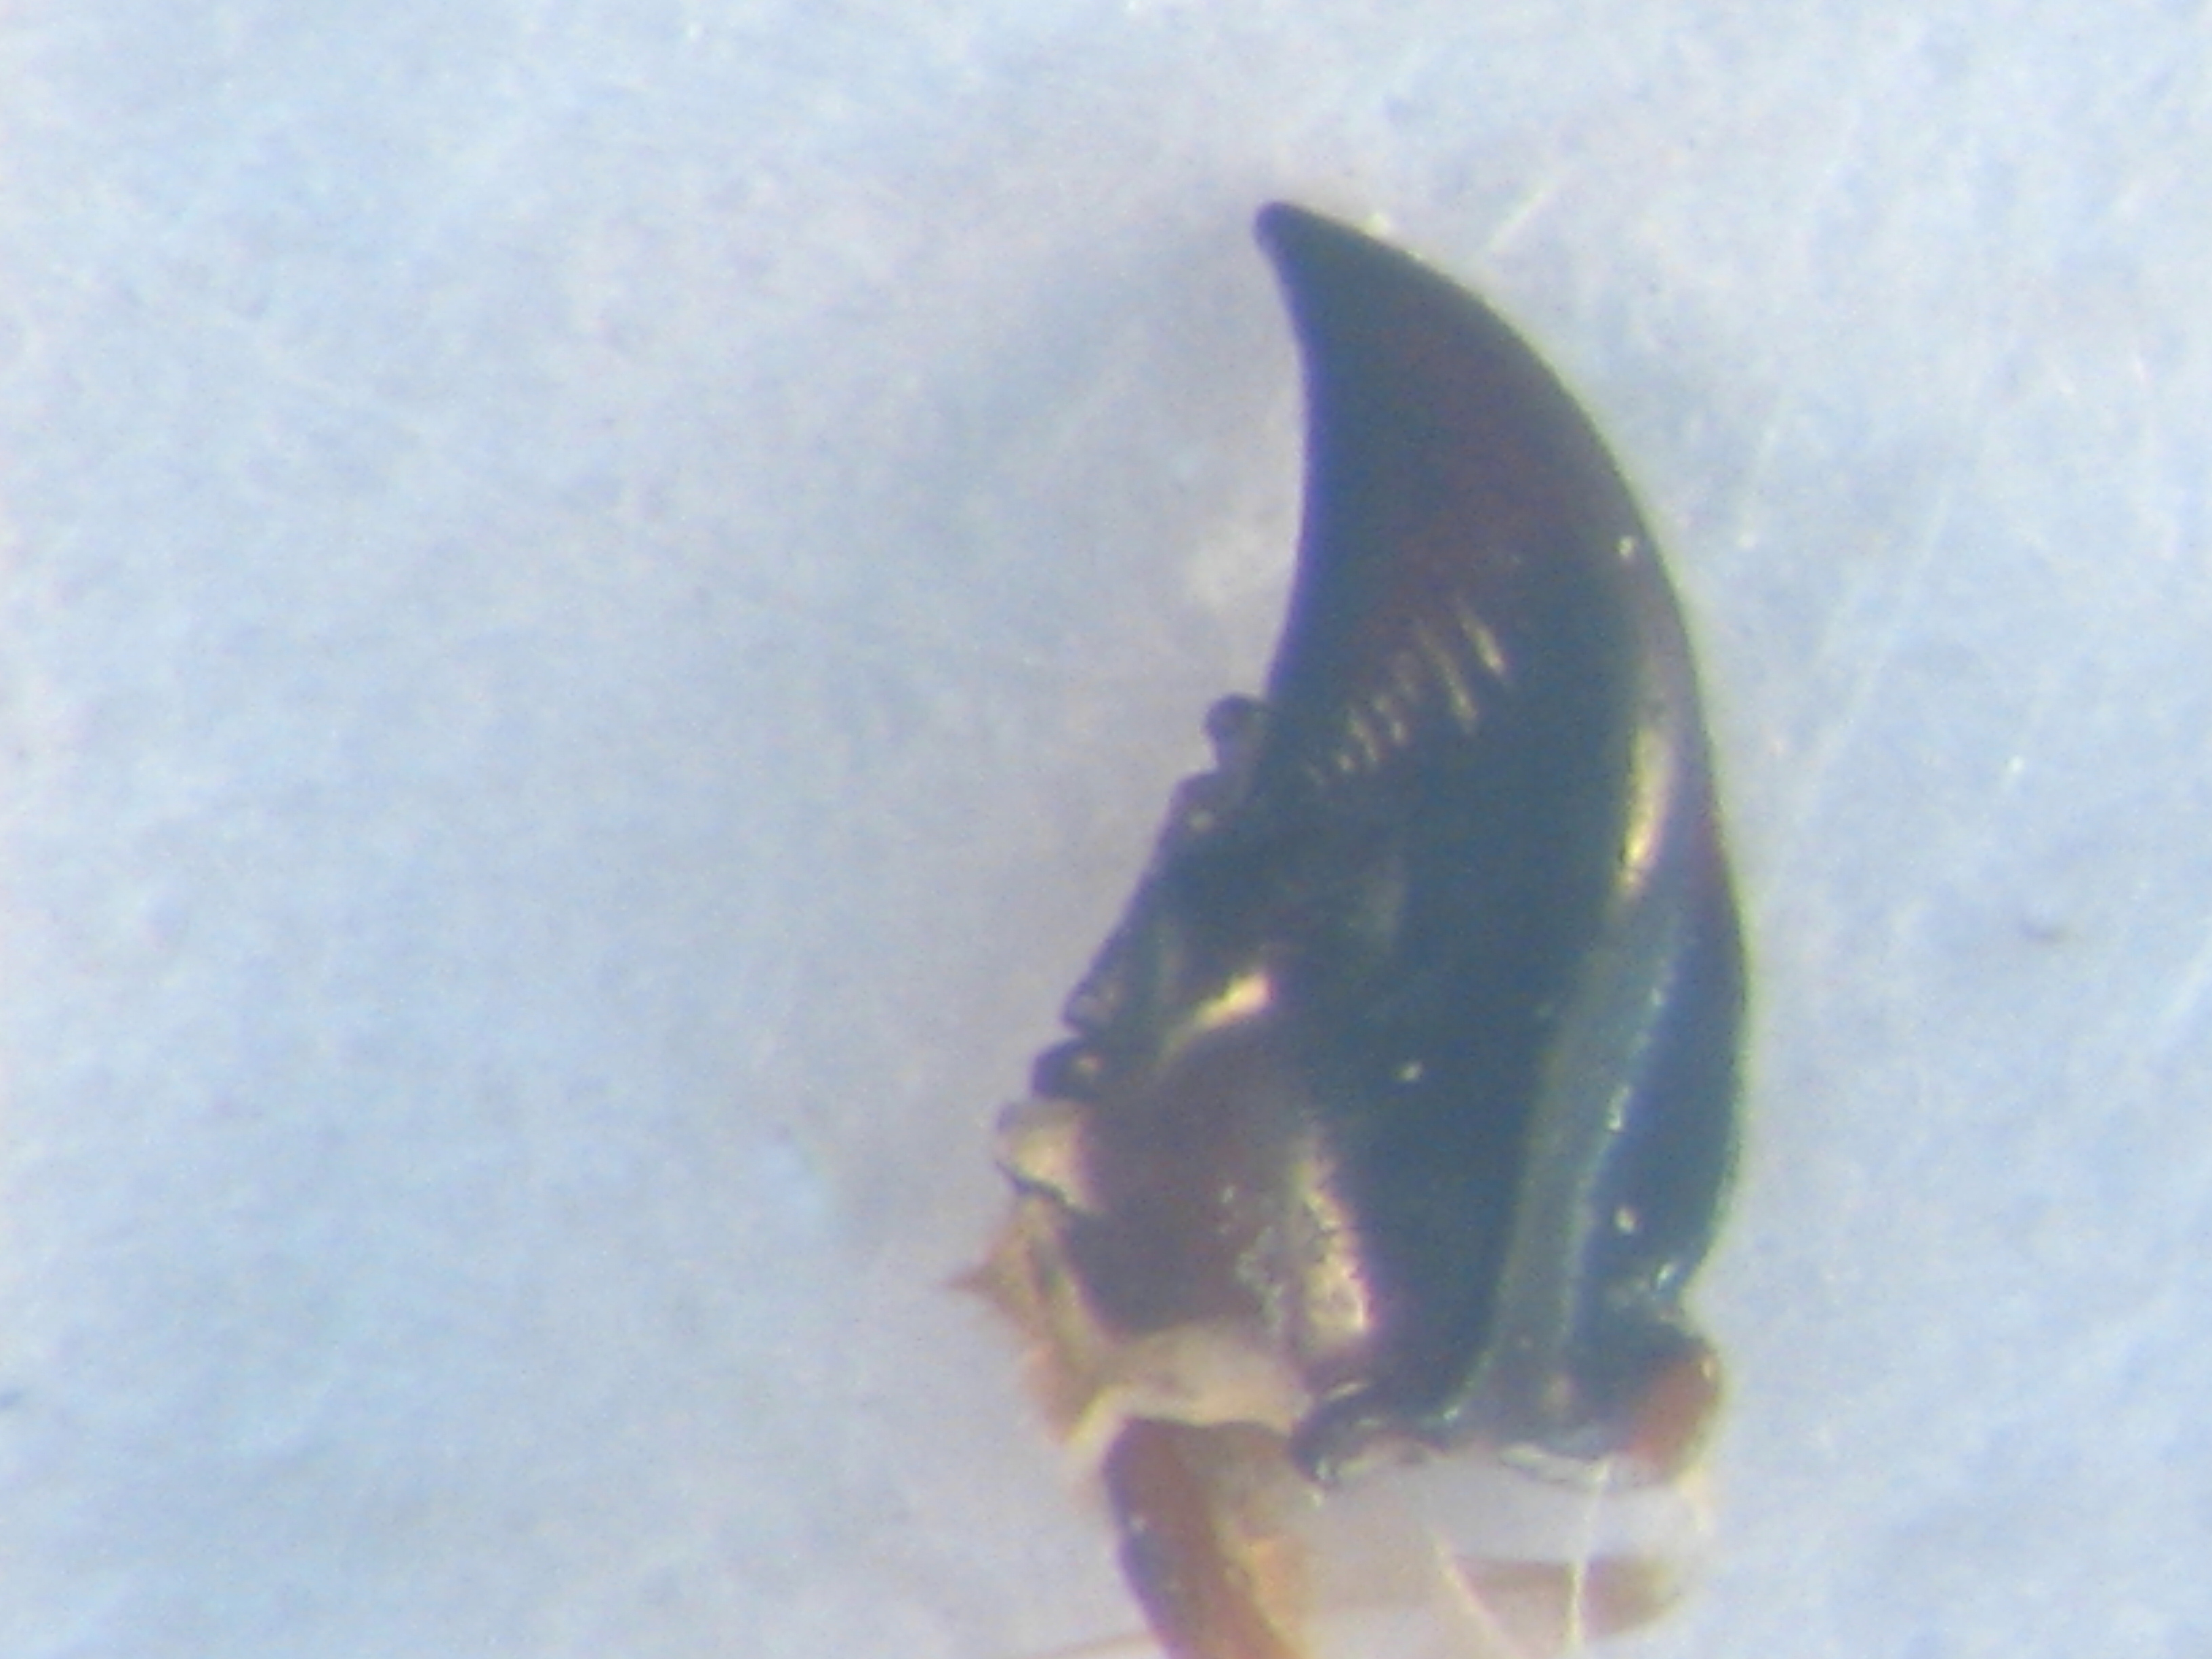
\includegraphics[width=0.45\textwidth]{./images/md019no}}~~
\subfloat[Image with line segmentation]{\label{fig:seg_222}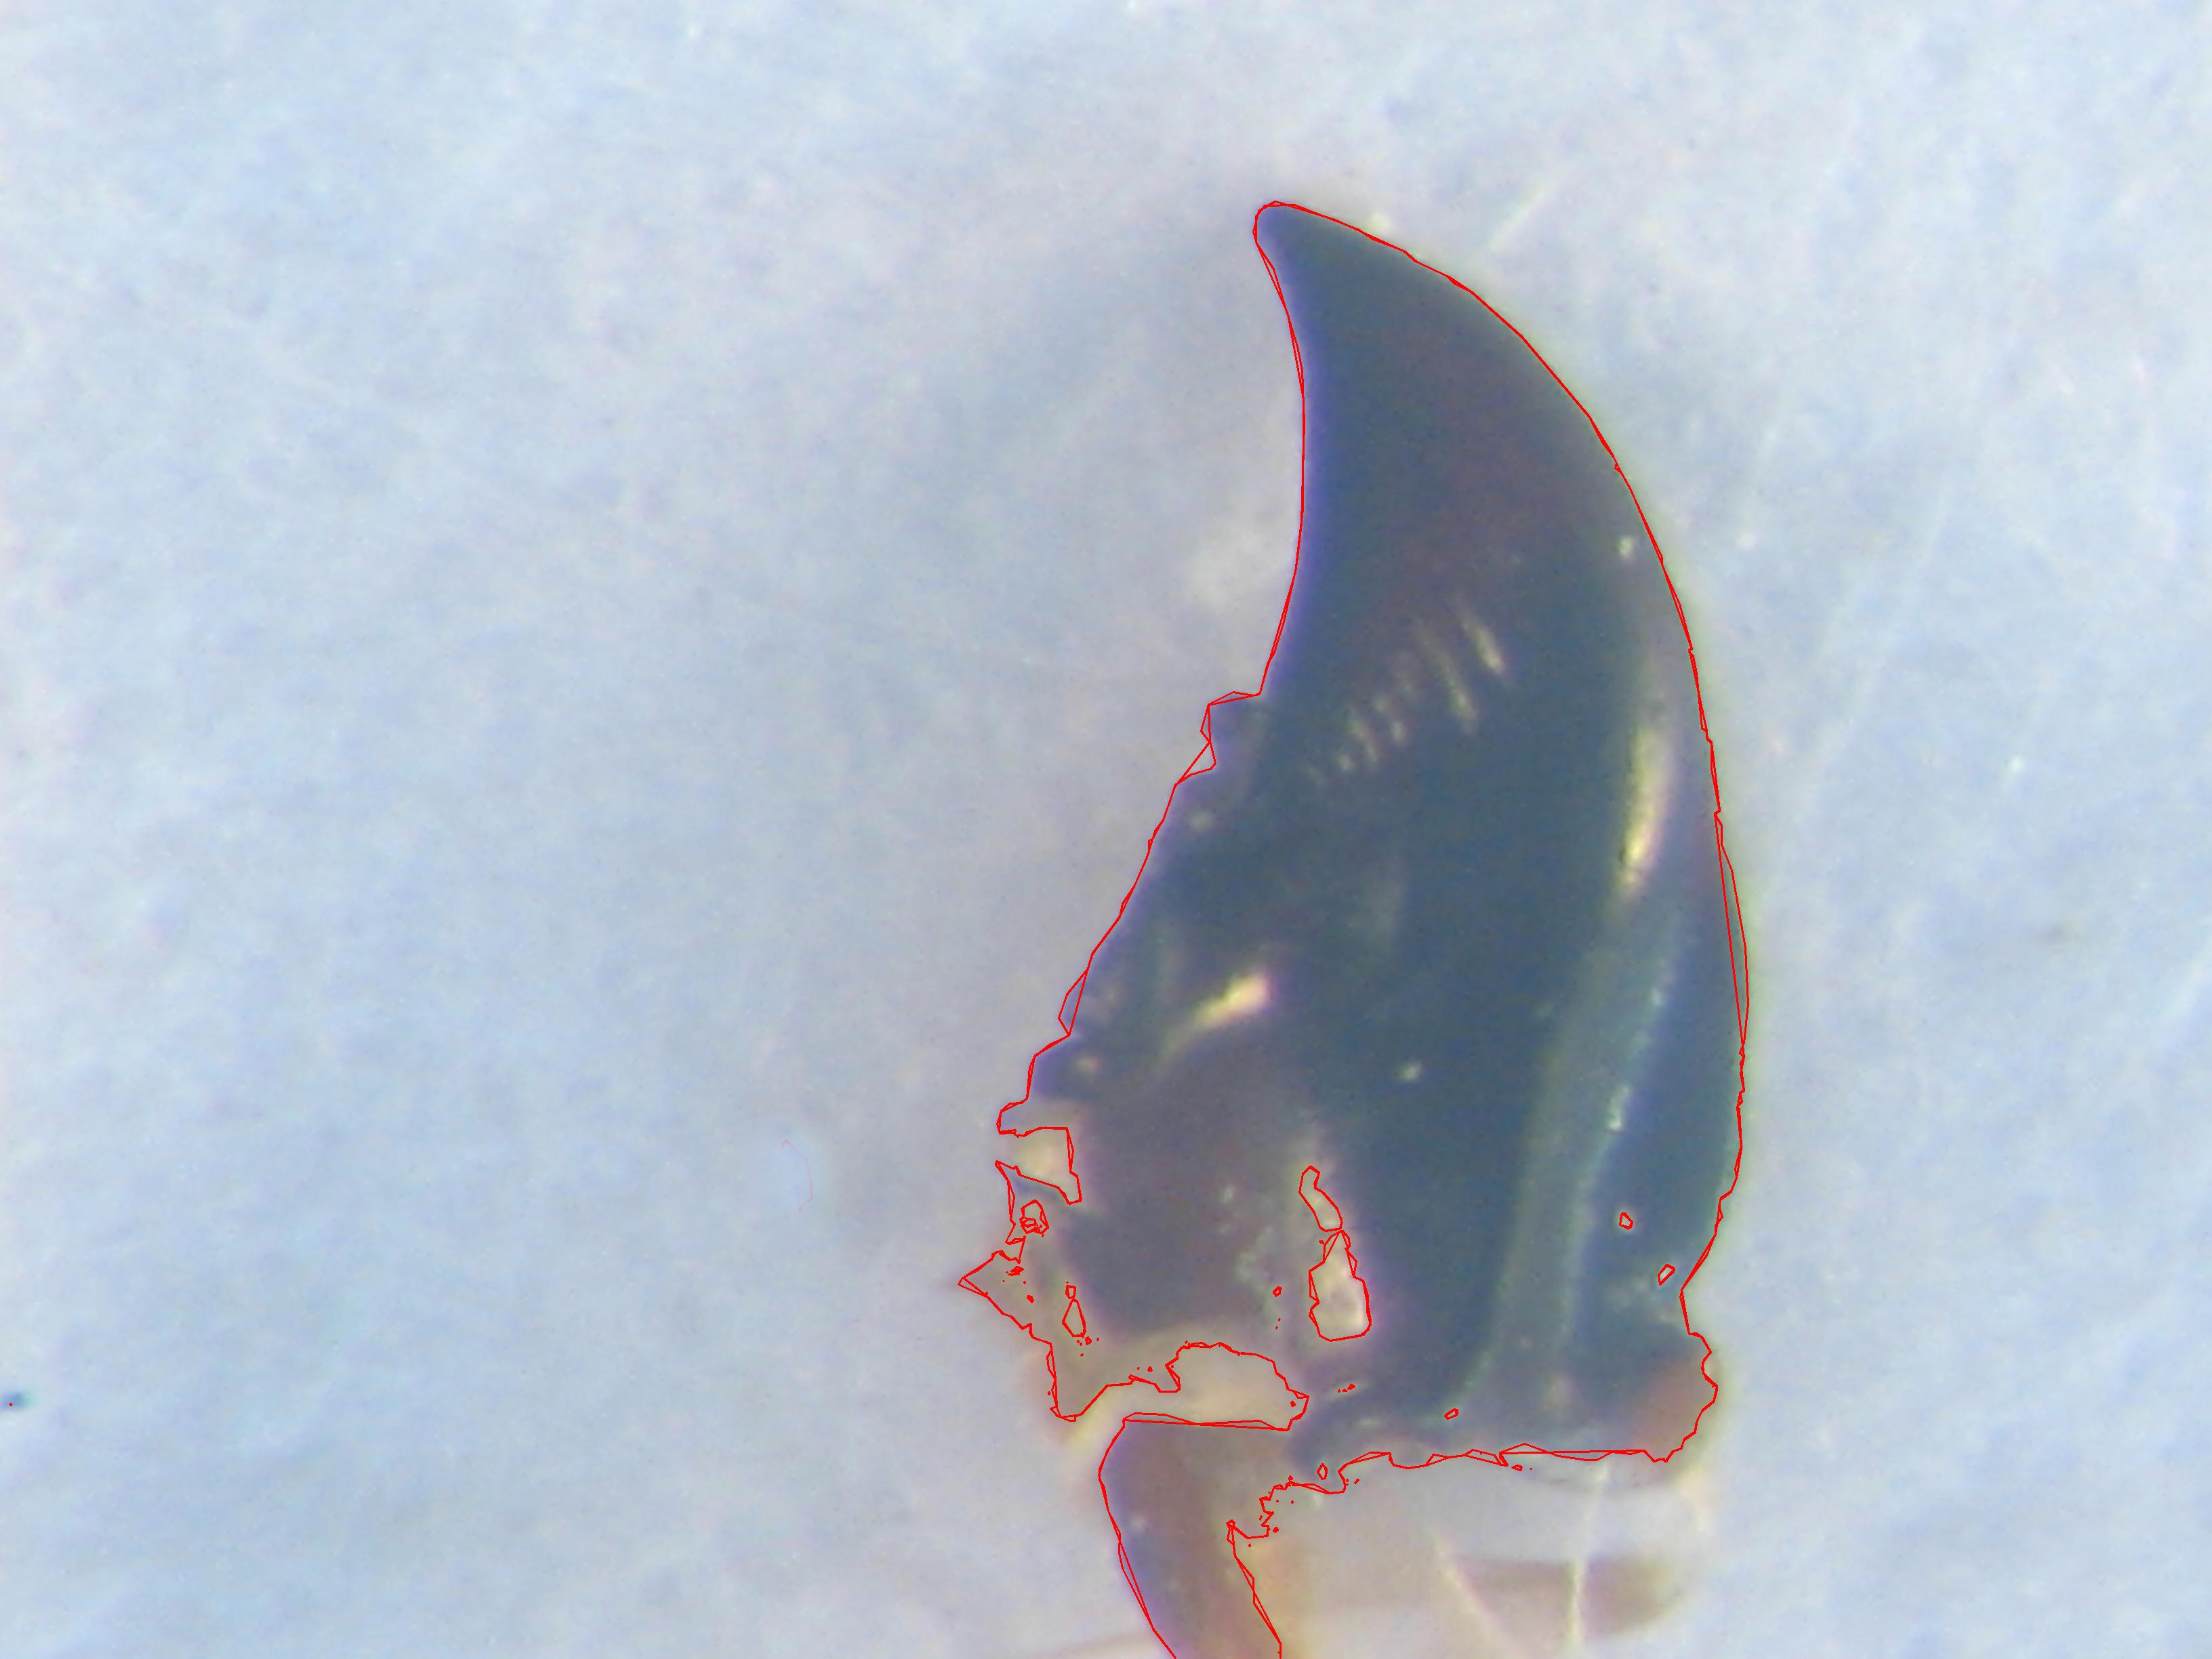
\includegraphics[width=0.45\textwidth]{./images/md019seg}}
\caption{An example about image segmentation}
\label{fig:figure_22}
\end{figure}
\section{Pairwise Geometric Histogram}
Pairwise Geometric Histogram(PGH)\cite{evans1993use} is used to encode the relative information between a line and a set of lines in an object. Therefore, an object can be represented by a set of PGHs. From the set of PGHs, we can reconstruct the object or compare it to another object. In this section, we introduce the construction of a PGH for an object based on the geometrical relationship and compute the similar distance between two objects. The object is described by set of approximate lines which were obtained in the previous stage.\\
The PGH is constructed based on the geometric features between lines relative. The geometric features are characteristics which can describe the geometric shape such as angle, the length of line, perpendicular distance between two lines, etc. For the shape representation, the relative angle and perpendicular distance is geometrical features useful.\\
\begin{figure}[h!]
\centering
\subfloat[The geometric relationship between two lines]{\label{fig:231}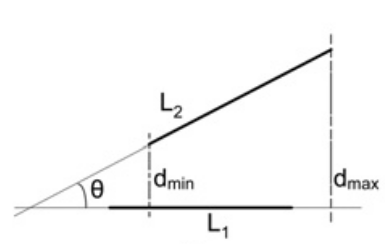
\includegraphics[width=0.4\textwidth]{./images/PGH_geo}}~~
\subfloat[The pairwise geometric histogram ]{\label{fig:232}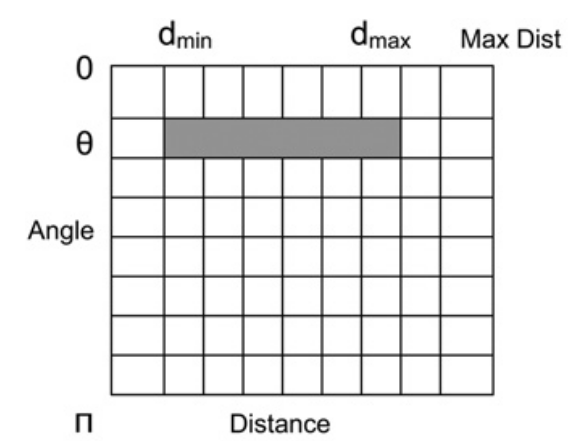
\includegraphics[width=0.4\textwidth]{./images/PGH}}
\caption{Example about geometric features and the pairwise geometric histogram\cite{palaniswamy2010automatic}}
\label{fig:figure_23}
\end{figure}
As example in figure \ref{fig:figure_23}\footnote{Image extracts from the article}, the figure \ref{fig:231} represents the geometric relationship between two lines \textbf{L1, L2}. The figure \ref{fig:232} represents the PGH between them when using line \textbf{L1} as reference line and line \textbf{L2} as object line.
\subsection{Local pairwise geometric histogram}
The local PGH presented the relationship between a reference line with other lines of the object. Thus, for each line in object, we can construct a local PGH for it. The frequency of the geometric features is recorded as a two dimensional histogram with an angle axis and distance axis. The entries on PGH describes the geometric relationship between the reference line and the object lines. \textit{``The blurring of entry along the axis regarding the true position and orientation of each object lines for reference line"}\cite{palaniswamy2010automatic}. Following the accuracy, we can indicate the size of histogram and normalize the value to match with size of histogram.
\subsection{Global pairwise geometric histogram}
Based on local PGH constructor, global PGH is combined of all local PGHs of all lines belong to the object. It means if the object is defined by $n$ lines, the global PGH will composed of $n$ local PGHs. This method fitwell when we apply some variants on the image, such as translate or rotate the image because the angle and perpendicular distance between a pair of lines are invariant.
\subsection{Histogram matching}
\textit{``The histogram matching enables robust classification of shape features by finding similarity between the scene and reference model"}\cite{palaniswamy2010automatic}. The similarity between two models can be obtained via the similar distance, which is computed by comparing their probability distribution on geometric histogram. To solve it, each model is represented by a global PGH and uses the Bhattacharya\cite{thacker1995assessing} metric to determine the similar distance between the two models \cite{palaniswamy2010automatic}. In general, we normalize the PGH before comparing. The form of Bhattacharrya metric used to compute the similarities between two models is:
\begin{center}
\begin{equation} \label{eq:1}
d_{Bhattacharyya} (H_{i}H_{j}) = \sum\limits_{\theta}^{\pi}\sum\limits_{d}^{d_{max}}\sqrt{H_{i}(\theta,d)H_{j}(\theta,d)}
\end{equation}
\end{center}
The significance of parameters in the formula \ref{eq:1}, as follows:
\begin{itemize}
\item $\theta$: angle value, range of $\theta$ in angle axis from 0 to $\pi$.
\item $d$: the perpendicular distance, range of $d$ in perpendicular distance from 0 to the maximum distance of arbitrary lines of shape.
\item $H_{i}(\theta,d)$ is an entry at row $\theta$ and column $d$ in PGH of image \textit{i}
\item $H_{j}(\theta,d)$ is an entry at row $\theta$ and column $d$ in PGH of image \textit{j}
\end{itemize}
\section{Probabilistic Hough Transform}
\textbf{Hough transform} is a technique used to find the presence of an object in another one. The main idea of this method is based on the \textit{``vote"} procedure. The Hough transform was originally developed to recognize a line\cite{hough1962method} and after, it has extended to apply on arbitrary shape\cite{duda1972use}.\\[0.2cm]
It exist a \textbf{Generalised Hough Transform}\cite{ballard1981generalizing} (GHT) which is the extension of Hough transform. It can be used to detect an object described with its model. The problem solved with GHT is finding the model's position in the image. Like \textbf{Hough transform}, GHT also use the vote procedure to solve the problem. Following the similarity metric (by Bhattacharya), the hypothesised matches can be used as input in pose estimation algorithm. But in the Palaniswamy's method, it is not used. They choose to use Probabilistic Hough Transform to estimate the global pose of the object\cite{ashbrook1995robust}.\\[0.3cm]
The PHT based on a group of features within the scene image, identifying the represent of a model image in a scene image. The hypothesised location of the model image in the scene image is indicated based on the conditional probability that any pair scene lines agreement about a position in model image.\\[0.3cm]
Estimating the global pose of the object has two main steps. Firstly, training process starts with recording the perpendicular distance and the angle from a reference point to each pair of model lines, then finding the similar pairs between model image and scene image. Secondly, estimating process starts as predicting the pose of scene image different from the model image, then we estimate the location of the model landmarks on scene image.
\subsection{Training process}
The training process begin with choosing a reference point in model. This point can be chosen at arbitrary position on the model image. At this step, the perpendicular distance and angle from each pair model lines to a reference point was recording and saving (called reference table). \\
To finish the training process, we find the presence of the model in the scene image by PHT. For each pair of scene lines, we find the pair of model lines (in reference table) which similar with the pair of scene lines and increase the value in accumulator at respectively location. The accumulator is a two-dimension matrix, one axis presents for angle, the other axis presents for the perpendicular distance. Finally, we choose the similar pair between model image and scene image. The chosen pair of scene lines is obtained from best votes in accumulator when we consider the similarity between each pair of scene image and model image.
\subsection{Estimating process}
The estimating process estimates the model's landmarks in scene's landmarks. Firstly, we estimate the position of model's reference point on scene image. Secondly, we estimate the model's landmarks on the scene image from the position of model's reference point in the scene image (figure \ref{fig:24}).
\begin{figure}[h!]
\centering
\subfloat[The model image]{\label{fig:241}
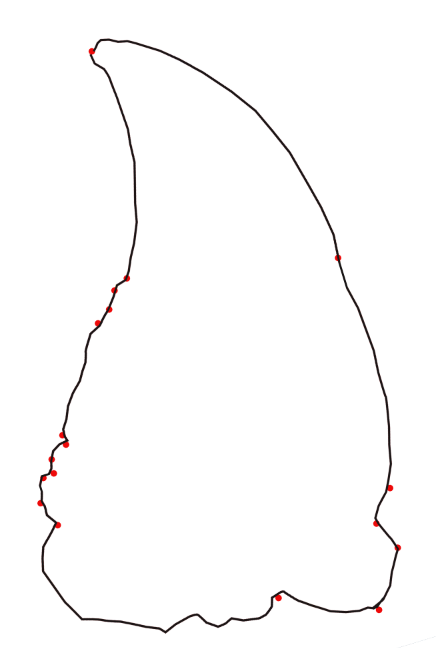
\includegraphics[width=0.3\textwidth]{./images/rshape}}~~
\subfloat[The scene image ]{\label{fig:242}
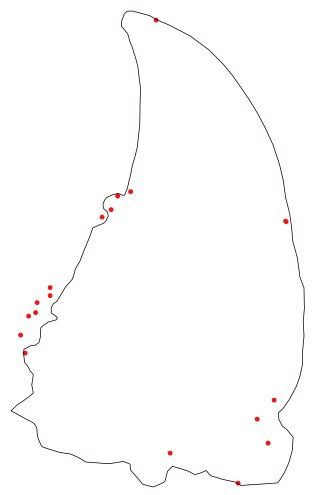
\includegraphics[width=0.3\textwidth]{./images/training}}
\caption{The landmarks estimated by Probabilistic Hough Transform}
\label{fig:24}
\end{figure}~\\
With a pair of scene lines agree with a pair of model lines chosen at previous step, the model's reference point in the scene image can be detected by extending the perpendicular lines of the pair of scene lines at the appropriate position\cite{ashbrook1995robust}.\\[0.2cm]
So, the estimation of model's landmarks in the scene image is estimated by calculating the relatedness between the model's reference point and the model's landmarks. Besides, we also record the difference about rotation, orientation and scale between the model image and the scene image.
In figure \ref{fig:24}, we apply the PHT to estimate the landmarks of the model to the scene. The image in figure \ref{fig:241} is the model. The image in figure \ref{fig:242} is scene. By applying the PHT, we estimate model's landmarks in the scene image as figure \ref{fig:242} (red points).
\section{Template matching}
Template matching is the process to refine the estimated landmarks, which was obtained by PHT of the scene image with an appropriate method. In the scope of this method, we use the cross-correlation to refine the estimated landmarks from PHT stage.\\[0.2cm]
Cross-correlation is a method of estimating the similarity between the two signals (searching a short signal in a long signal). By computing the sum of products between two signals when a signal is sliding on another signal. The position is considered similar if the value at this position is maximal. In image processing, it is used to detect the present of an object (template) in a large object (image). The equation of cross-correlation is as follows (equation \ref{eq:cross-correlation}):
\begin{center}
\begin{equation}\label{eq:cross-correlation}
R_{ccorr}(x,y) = \sum\limits_{x',y'}[T(x'.y').I(x + x', y + y')]
\end{equation}
\end{center}
Where:
\begin{itemize}
\item T is template which use to slide and find the exist in other image.
\item I is image which we expect to find the template image
\item $(x', y')$ are coordinates in template where we get the value to compute.
\item $(x + x', y + y')$ are coordinates in image where we get the value to compute when template $T$ sliding.
\end{itemize}
By sliding the template on image by each pixel from left to right and top to down. At each position, we compute the $R_{ccorr}(x,y)$. The position having maximal $R_{ccorr}(x,y)$ is the best similar of template in image.\\[0.2cm]
However, if we use the original image to compute and find the similarity, the brightness of the template and the image might change the conditions and the result. So, we can normalize the image before applying the cross-correlation to reduce the effect of lighting difference between them. The normalization coefficient is:
\begin{center}
\begin{equation}\label{eq:normalizeCoff}
Z(x,y) = \sqrt{\sum\limits_{x',y'}T(x'.y')^{2}.\sum\limits_{x',y'}I(x + x', y + y')^{2}}
\end{equation}
\end{center}
The value of this method when we normalized computation as below:
\begin{center}
\begin{equation}\label{eq:cross-correlation}
R_{ccorr\_norm}(x,y) =\frac{R_{ccorr}(x,y)}{Z(x,y)} = \frac{\sum\limits_{x',y'}[T(x'.y').I(x + x', y + y')]}{\sqrt{\sum\limits_{x',y'}T(x'.y')^{2}.\sum\limits_{x',y'}I(x + x', y + y')^{2}}}
\end{equation}
\end{center}
\section{Summary}
This chapter describes the stages of the method \textbf{``Automatic identification of landmarks in digital images"}. In this present, we have changed some ways to suitable with our problems (beetles instead of fly) such as method to pre-process image, rate between the lower threshold and upper threshold value in Canny, etc. Next chapter will discuss about the algorithms to implement the Palaniswamy's method.